\section{Experiments}

\subsection{Experimental Setup}

We evaluate our method on the CO3Dv2 dataset, a large-scale benchmark containing multi-view video captures of real-world objects under diverse viewpoints and backgrounds. To stress-test reconstruction quality in challenging scenarios, we focus on categories such as Bowl and Teddy, which contain thin-walled structures, self-occlusions, and complex geometries.

\subsection{Preprocessing}

For each video sequence, frames are extracted at a fixed frame rate and camera intrinsics/extrinsics are estimated using COLMAP. Foreground object masks are generated with SAM2 using a single user-provided prompt on the first frame.

\subsection{Training Details}

We build our method on top of the original 3D Gaussian Splatting (3DGS) framework. During optimization, we apply the proposed Mask-Guided Compound Loss, which combines mask-constrained L1 supervision with a composite-image SSIM loss. The loss weights $\lambda_1$ and $\lambda_2$ are empirically set to balance photometric accuracy and structural consistency.

After reconstruction, we apply the proposed Geometry-Aware Multi-Metric Pruning procedure, including multi-view mask consistency checking, KNN-based density and anisotropy filtering, and adaptive shrinkage refinement.

\subsection{Baseline and Metrics}

We compare our method against original 3D Gaussian Splatting (3DGS) trained directly on the original video frames without segmentation guidance.

We report the following metrics to evaluate reconstruction quality:

\begin{itemize}
    \item PSNR (Peak Signal-to-Noise Ratio)
    \item SSIM (Structural Similarity Index)
    \item LPIPS (Learned Perceptual Image Patch Similarity)
\end{itemize}

In addition, we provide qualitative comparisons focusing on background suppression, boundary sharpness, and the removal of floating artifacts.

\subsection{Quantitative Results}

Table~\ref{tab:main} reports quantitative results on representative CO3Dv2 sequences.

\begin{table}[t]
\centering
\caption{Quantitative comparison on CO3Dv2 sequences.
Metrics are evaluated within foreground mask regions.}
\label{tab:main}
\begin{tabular}{lccc}
\toprule
Method & PSNR$\uparrow$ & SSIM$\uparrow$ & LPIPS$\downarrow$\\
\midrule
Original 3DGS & 19.07 & 0.592 & 0.629 \\
Mask-Guided & 21.03 & 0.931 & 0.125 \\
MOF3R (ours) & \textbf{23.56} & \textbf{0.935} & \textbf{0.120} \\
\bottomrule
\end{tabular}
\end{table}

Figure~\ref{fig:result} visualizes the quantitative performance in different object sequences. The proposed pipeline consistently improves perceptual quality while maintaining
high structural similarity.

\begin{figure}
    \centering
    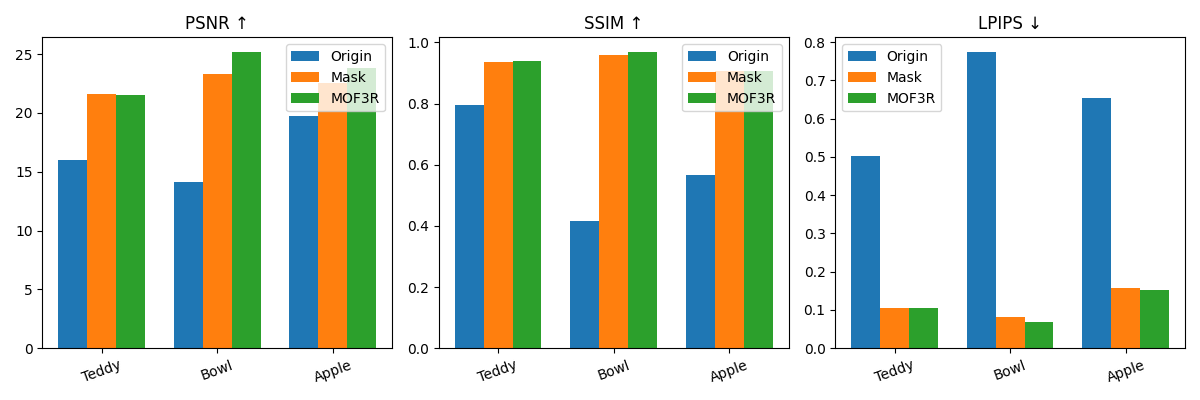
\includegraphics[width=\linewidth]{pics/result.png}
    \caption{Comparison of reconstruction quality across representative
CO3Dv2 sequences.}
    \label{fig:result}
\end{figure}

Compared with original 3DGS, our full pipeline improves the average PSNR from 19.07 dB to 23.56 dB and reduces LPIPS from 0.629 to 0.120. These improvements indicate that semantic guidance effectively suppresses background fitting while geometric pruning removes residual artifacts.

The proposed geometry-aware pruning stage further improves reconstruction quality by removing residual floating artifacts and elongated Gaussian primitives. The improvements are particularly evident on challenging objects such as Bowl, where the full pipeline improves PSNR from 14.10 dB to 25.17 dB while reducing LPIPS from 0.774 to 0.068.

Full per-sequence quantitative results, including different pruning configurations and training iterations, are provided in Appendix~\ref{sec:full_result}.

\subsection{Qualitative Results}

Figure~\ref{fig:qualitative} presents qualitative
comparisons on representative CO3Dv2 scenes. Qualitative comparisons further demonstrate cleaner object boundaries, fewer background artifacts, and more compact Gaussian distributions, validating the complementary benefits of semantic guidance and geometric refinement.

Without foreground supervision, original 3DGS tends to allocate Gaussian primitives to background regions, resulting in severe floating artifacts and blurred object boundaries.

By introducing the proposed mask-guided loss, the optimization process becomes object-centric and substantially suppresses background interference. However, a small number of residual artifacts remain around object boundaries.

The proposed geometry-aware pruning stage further removes isolated and elongated Gaussian primitives, producing cleaner silhouettes and more compact reconstructions. The improvement is particularly visible on the TeddyBear, Bowl, and Apple scenes, where boundary sharpness and visual consistency are significantly enhanced.

\begin{figure*}[t]
    \centering
    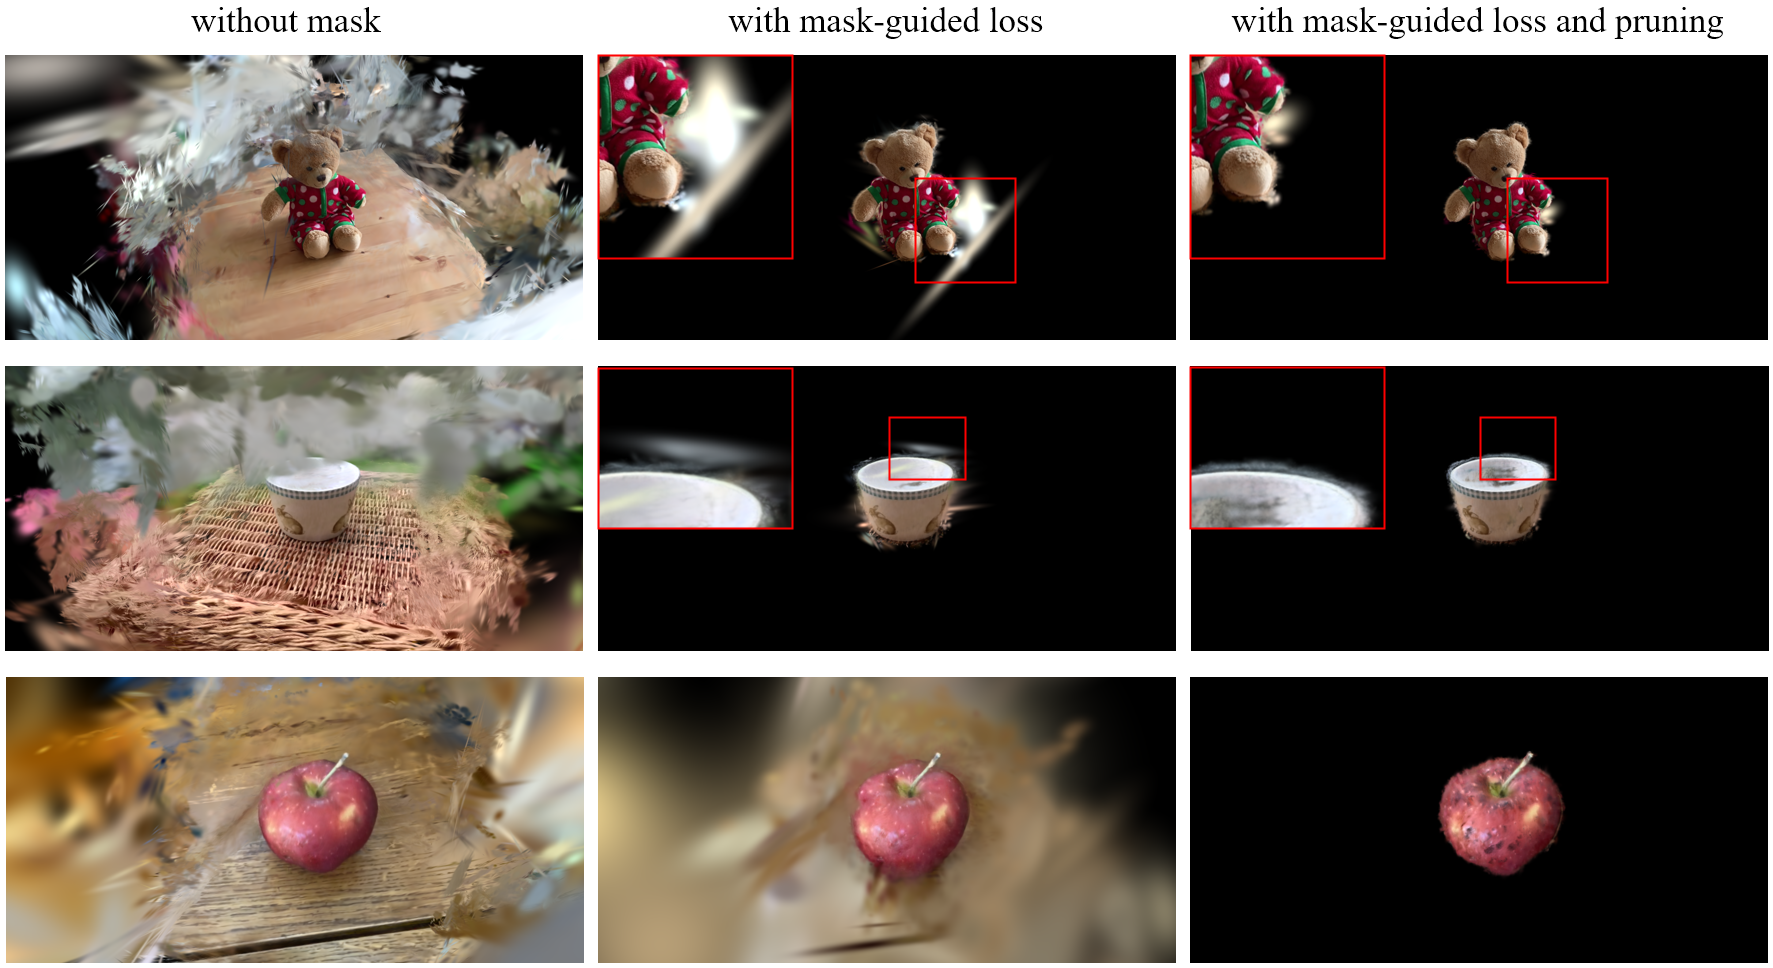
\includegraphics[width=\textwidth]{pics/comparsion.png}
    \caption{
    Qualitative comparison of reconstruction results.
    From left to right: original 3DGS, reconstruction with the proposed mask-guided loss, and the full MOF3R pipeline with geometry-aware pruning.
    The mask-guided loss effectively suppresses background interference, while the pruning stage further removes floating artifacts and improves object boundary quality.
    }
    \label{fig:qualitative}
\end{figure*}

\subsection{Ablation Study}

We conduct an ablation study to evaluate the contribution of each component in the proposed pipeline.

Starting from original 3DGS, we first introduce the mask-guided compound loss, which restricts optimization to foreground regions. We then apply the proposed geometry-aware pruning strategy to remove residual artifacts and elongated Gaussian primitives.

Results in Table~\ref{tab:ablation} show that the pruning stage further improves reconstruction quality by removing floating artifacts and refining object boundaries where Reasonable pruning showcases the best performance.

\begin{table}[t]
\centering
\caption{Effect of different pruning strategies.}
\label{tab:ablation}
\begin{tabular}{lccc}
\toprule
Pruning Type & PSNR$\uparrow$ & SSIM$\uparrow$ & LPIPS$\downarrow$\\
\midrule
None & 21.03 & 0.931 & 0.125\\
Conservative & 23.18 & 0.933 & 0.123\\
Reasonable & \textbf{23.56} & \textbf{0.935} & \textbf{0.120}\\
Aggressive & 23.42 & 0.932 & 0.121\\
\bottomrule
\end{tabular}
\end{table}

